% A morphism pi: X -> Y of ringed spaces, with an open U in Y and its preimage in X.
% Source: book/tex/alg-geom/mor-scheme.tex (§ morphisms of ringed spaces).
\documentclass[border=2mm]{standalone}
\usepackage{amsmath}\usepackage{amssymb}\usepackage{tikz}
\usetikzlibrary{arrows.meta}
\begin{document}
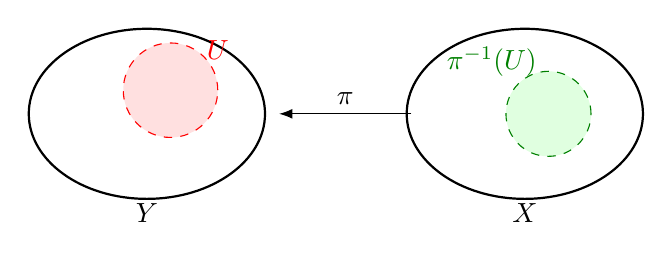
\begin{tikzpicture}[scale=0.6]
  \draw[thick] (-6,0) ellipse (2.5 and 1.8);
  \node at (-6,-2.1) {$Y$};
  \draw[red,dashed,fill=red!12] (-5.5,0.5) circle (1);
  \node[red] at (-4.5,1.35) {$U$};
  \draw[thick] (2,0) ellipse (2.5 and 1.8);
  \node at (2,-2.1) {$X$};
  \draw[green!50!black,dashed,fill=green!12] (2.5,0) circle (0.9);
  \node[green!50!black] at (1.3,1.1) {$\pi^{-1}(U)$};
  \draw[-{Latex}] (-0.4,0) -- (-3.2,0) node[midway,above] {$\pi$};
\end{tikzpicture}
\end{document}
